\documentclass{beamer}
\usetheme{default}


\title{ECE411 Final Presentation}
\subtitle{Womprats T-16 Audio Synthesizer}
\author{A. Goetz \and B. Kanyid \and J. Pugh \and K. Riedl}
\institute[PSU]{
  Maseeh College of Engineering and Computer Science\\
  Portland State University\\
  Portland, Oregon 97207  
}
\date{\today}


\begin{document}
\begin{frame}[plain]
  \titlepage
\end{frame}



\begin{frame}{Problem}

  \textbf{Problem Statement:}  \pause Build something cool in order to
  practice for engineering capstone. 

  \pause \textit{Okay, what really is the goal of this project?}

  \pause Use both hard engineering and soft people skills to
  successfully develop a product in a ten week period. 
  
  \pause \textit{Yeah, but what did you actually build?}

  \pause Design and implement a multi-channel audio-synthesizer for
  chiptune music.

  
\end{frame}

\begin{frame}{Motivation}
%% Why is it important? What is the value of a solution (lives, money,
%% effort, energy saved)?

  Our solution provides a simple interface that allows the generation
  of complex waveforms. 

  On a higher level, it demonstrates that we can balance real-world
  engineering tradeoffs in a practical project. 

\end{frame}

\begin{frame}{Objective}

  Our objective is to design, build and test an audio synthesizer
  capable of mixing multiple waveforms to create a single audio out. 
\end{frame}

\begin{frame}{Alternatives}
%% How is it done today or what other alternatives exist?

There are many synthesizer products on the market today. Our goal is
not to compete with these products, but to create something that is realizable in 10 weeks. 
\end{frame}

\begin{frame}{Requirements}
%% What are the requirements for an acceptable solution?  

\end{frame}

\begin{frame}{Our Approach}
Brief overview of your approach
\end{frame}

\begin{frame}{Design}
May need multiple sub-headings here (e.g.  H/W and S/W, or multiple
subsystems) Describe design using appropriate methods (e.g.  UML
models, algorithms) Discuss design alternatives, trade-offs, decisions
made
\end{frame}

\begin{frame}{Implementation}
Details of implementation (major components, schematics, board layout,
code)	  
Tools employed (e.g.  simulation/modeling tool, PCB layout, IDE,
cross-compilers)
\end{frame}

\begin{frame}{IP and Prior Work}
Brief summarize what use you made of prior work or IP including but
not limited to ideas, designs, schematics, board layouts, code.
\end{frame}

\begin{frame}{Testing}
What was the testing strategy and plan?  
\end{frame}

\begin{frame}{Results}
What worked? How well? What didn't? Why?
  
\end{frame}

\begin{frame}{Contributions}
What were the contributions of each member (e.g.  who did PCB, coding,
testing, writing)?
  
\end{frame}
\begin{frame}{Lessons Learned}
\end{frame}

\begin{frame}{PCB}
\end{frame}
%\frame{\titlepage}
\frame{\frametitle{Agenda}\tableofcontents} 


% 30 seconds for overview
\section{Project Overview} 
\frame{\frametitle{Project Overview} 
[Overview text here]
Audio synthesizers provide entertainment by creating unique sounds.
}
\subsection{Objective}
\frame{{Objective}
[Objective text here]
Design and build a device that can generate sounds from user-control.
}
\subsection{Requirements}
\frame{{Requirements}
\begin{itemize}
\item Avoid  mechanical complexity
\item Make the project cheap enough to replicate for each of us to have one / make one cheaply
\item Stick to free/open source software if possible
\item Stick to cheap hardware tool costs if possible (try not to buy tools)
\item Project should be gracefully degradable, i.e. modular (so if we need to cut corners it won't cause complications)
\item Keep logic "breadboardable" i.e. keep it simple enough to prototype on a breadboard
\item Use plug and play devices if possible
\item Device should be safe for the user and durable
\item Suitable for bringing into an interview situation (keep it portable)
\end{itemize}

}
\subsection{Approach}
\frame{{Approach}
Project Management \& Documentation tools
\begin{itemize}
\item GanttProject
\item Redmine
\item \LaTeX
\end{itemize}

Technical tools
\begin{itemize}
\item KiCad EDA
\item LPCXpresso Code Red IDE
\item Git
\end{itemize}
}

\section{Design}
\frame{\frametitle{Design}
[Design text here]\\

  \begin{figure}[htb]
    \centering
    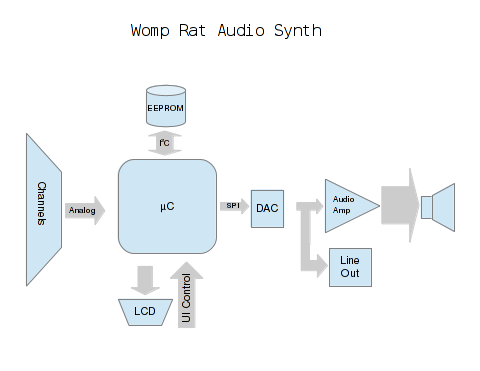
\includegraphics[width=0.7\textwidth]{BlockLevelDiagram.png} 
    \caption{Block Diagram Overview}
  \end{figure}

}

\subsection{Implementation}
\frame{{Implementation}
The parts chosen for making the audio synthesizer:
\begin{itemize}
  \pause
\item Microcontroller: NPX LPC 1114
  \pause
\item EEPROM: Atmel AT24C128C
  \pause
\item LCD: EA DOGS102W-6 +EA LED39x41-W
  \pause
\item Channels: 
  \pause
\item DAC: MCP4921
  \pause
\item Audio Amplifier: LM4875
\end{itemize}
}

\subsection{PCB Layout}
\frame{{PCB Layout} 

\begin{center}
 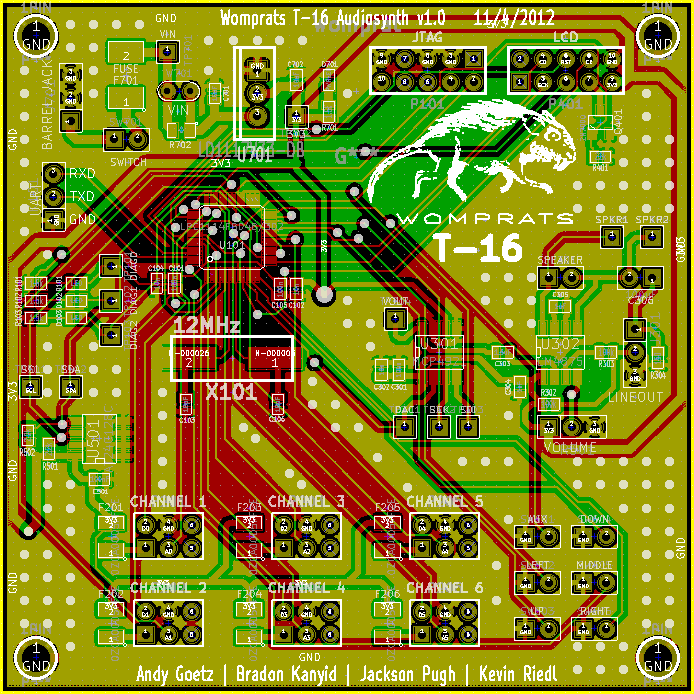
\includegraphics[width=0.7\textwidth]{pcb.png}
\end{center}
}


\begin{frame}{Lessons Learned}
\end{frame}
\subsection{Testing \& Debugging}
\frame{{Testing \& Debugging}
\begin{itemize}
  \pause
\item Microcontroller

  \begin{itemize}
    \pause
    \item Programming Test
    \pause
    \item Diagonistic Test
    \pause
    \end{itemize}
\item EEPROM
  \begin{itemize}
    \pause
    \item Read/Write Byte Test
    \pause
    \item Read/Write Burst Test
    \pause
    \end{itemize}
\item LCD
  \begin{itemize}
    \pause
    \item LCD Test
    \pause
    \item Button Test
    \pause
  \end{itemize}
\item DAC
  \begin{itemize}
    \pause
    \item I/O Test (DAC Test)
    \pause
    \end{itemize}
\item Audio Amplifier
  \begin{itemize}
    \pause
    \item Frequency Test
    \pause
    \item Line-out Test
    \pause
    \item Volume Control Test
    \pause
    \end{itemize}
\item Power Supply
  \begin{itemize}
    \pause
    \item Fuse Test
    \pause
    \item Voltage Ripple Test
    \pause
    \end{itemize}
\end{itemize}
}

\subsection{Integration Tests}
\frame{{Integration Tests}
\begin{itemize}
  \pause
  \item Power-On Self-Test
  \pause
  \item DAC-Audio Amplifier Test
  \pause
  \item Display Womprat on LCD screen
\end{itemize}
}

\subsection{Results}
\frame{{Results}
[Results text here]
}

\section{Team Evaluation}
\frame{\frametitle{Team Evaluation}
[Team Evaluation text here]
}
\subsection{Contributions}
\frame{{Contributions}
[Contributions text here]
}
\subsection{Lessons Learned}
\frame{{Lessons Learned}
  Bradon Kanyid

  Andy Goetz

  Kevin Riedl

  Jackson Pugh

}


%\section{Design Choices}
%\frame{\frametitle{Design Choices} 
%Design Choices text here
%}

%\begin{frame}{Design Choices}
%  \begin{itemize}
%    \pause
%  \item KiCad
%    \pause
%  \item LPC1114
%    \pause
%  \item GanttProject
%    \pause
%  \item \LaTeX
%    \end{itemize}
%\end{frame}



\end{document}
